\documentclass[12pt]{article}

\newdimen\mymargin
\setlength{\mymargin}{1.0in}

\usepackage[margin=\mymargin]{geometry}
\usepackage{xcolor}
\usepackage{ulem}
\usepackage{microtype}
\usepackage[ngerman]{babel}
\usepackage{tabularx}
\usepackage{enumitem}
\usepackage{graphicx}

% title
\title{\vspace{-100pt}\LARGE Lebenslauf\vspace{-18pt}}
\author{\LARGE Nicholas Schweitzer}
\date{}

% link and section macros
\newcommand{\link}[1]{{\color{blue}\underline{#1}}}
\newcommand{\sect}[1]{
  {
    \vspace{12pt}
    \section*{
      \fontsize{18}{0}\selectfont
      \hspace{-12pt}
      \vspace{-12pt}
      #1
    }
    \vspace{-6pt}
  }
}

% page formatting options
\setlength\parindent{0pt}
\setlength\parskip{7pt}
\pagenumbering{gobble}

% other commands
\newcommand{\sep}{{\color{gray}\vspace{-12pt}\hrule}}
\newcommand{\ask}[1]{{\color{red}#1}}

% main document
\begin{document}
\maketitle
\vspace{-32pt}

% \section*{Motivation}
% Ich bin Sch{\"u}ler in die 10. Klasse und bin in ein Praktikum bei DLR entweder in Oberpfaffenhofen oder Weilheim im Bereich von Aerodynamik und Raumfahrt interessiert. Technologie, Physik und Mathematik fand ich immer interessant und ich hoffe durch ein Praktikum bei DLR mein Wissen zu erweitern und praktische Erfahrung zu gewinnen sowie mit anderen {\"u}ber meine Interessen reden.

\begin{figure}[htb!]
  \begin{minipage}{0.7\textwidth}
    \textbf{Geburt} \hfill{27.09.2003} \, \\
    \sep
    \vspace{7pt}
    \textbf{Email} \hfill{nicholas\_schweitzer@mis-munich.de} \, \\
    \sep
    \vspace{7pt}
    \textbf{Mobil / Festnetz} \hfill{0176 8053 1248 / 08171 238 1130} \, \\
    \sep
    \vspace{7pt}
    \textbf{Adresse} \hfill{Am Haken 2, 82538 Geretsried \, }\\
    \sep
    \vspace{7pt}
  \end{minipage}
  \begin{minipage}{0.29\textwidth}
    \hfill
    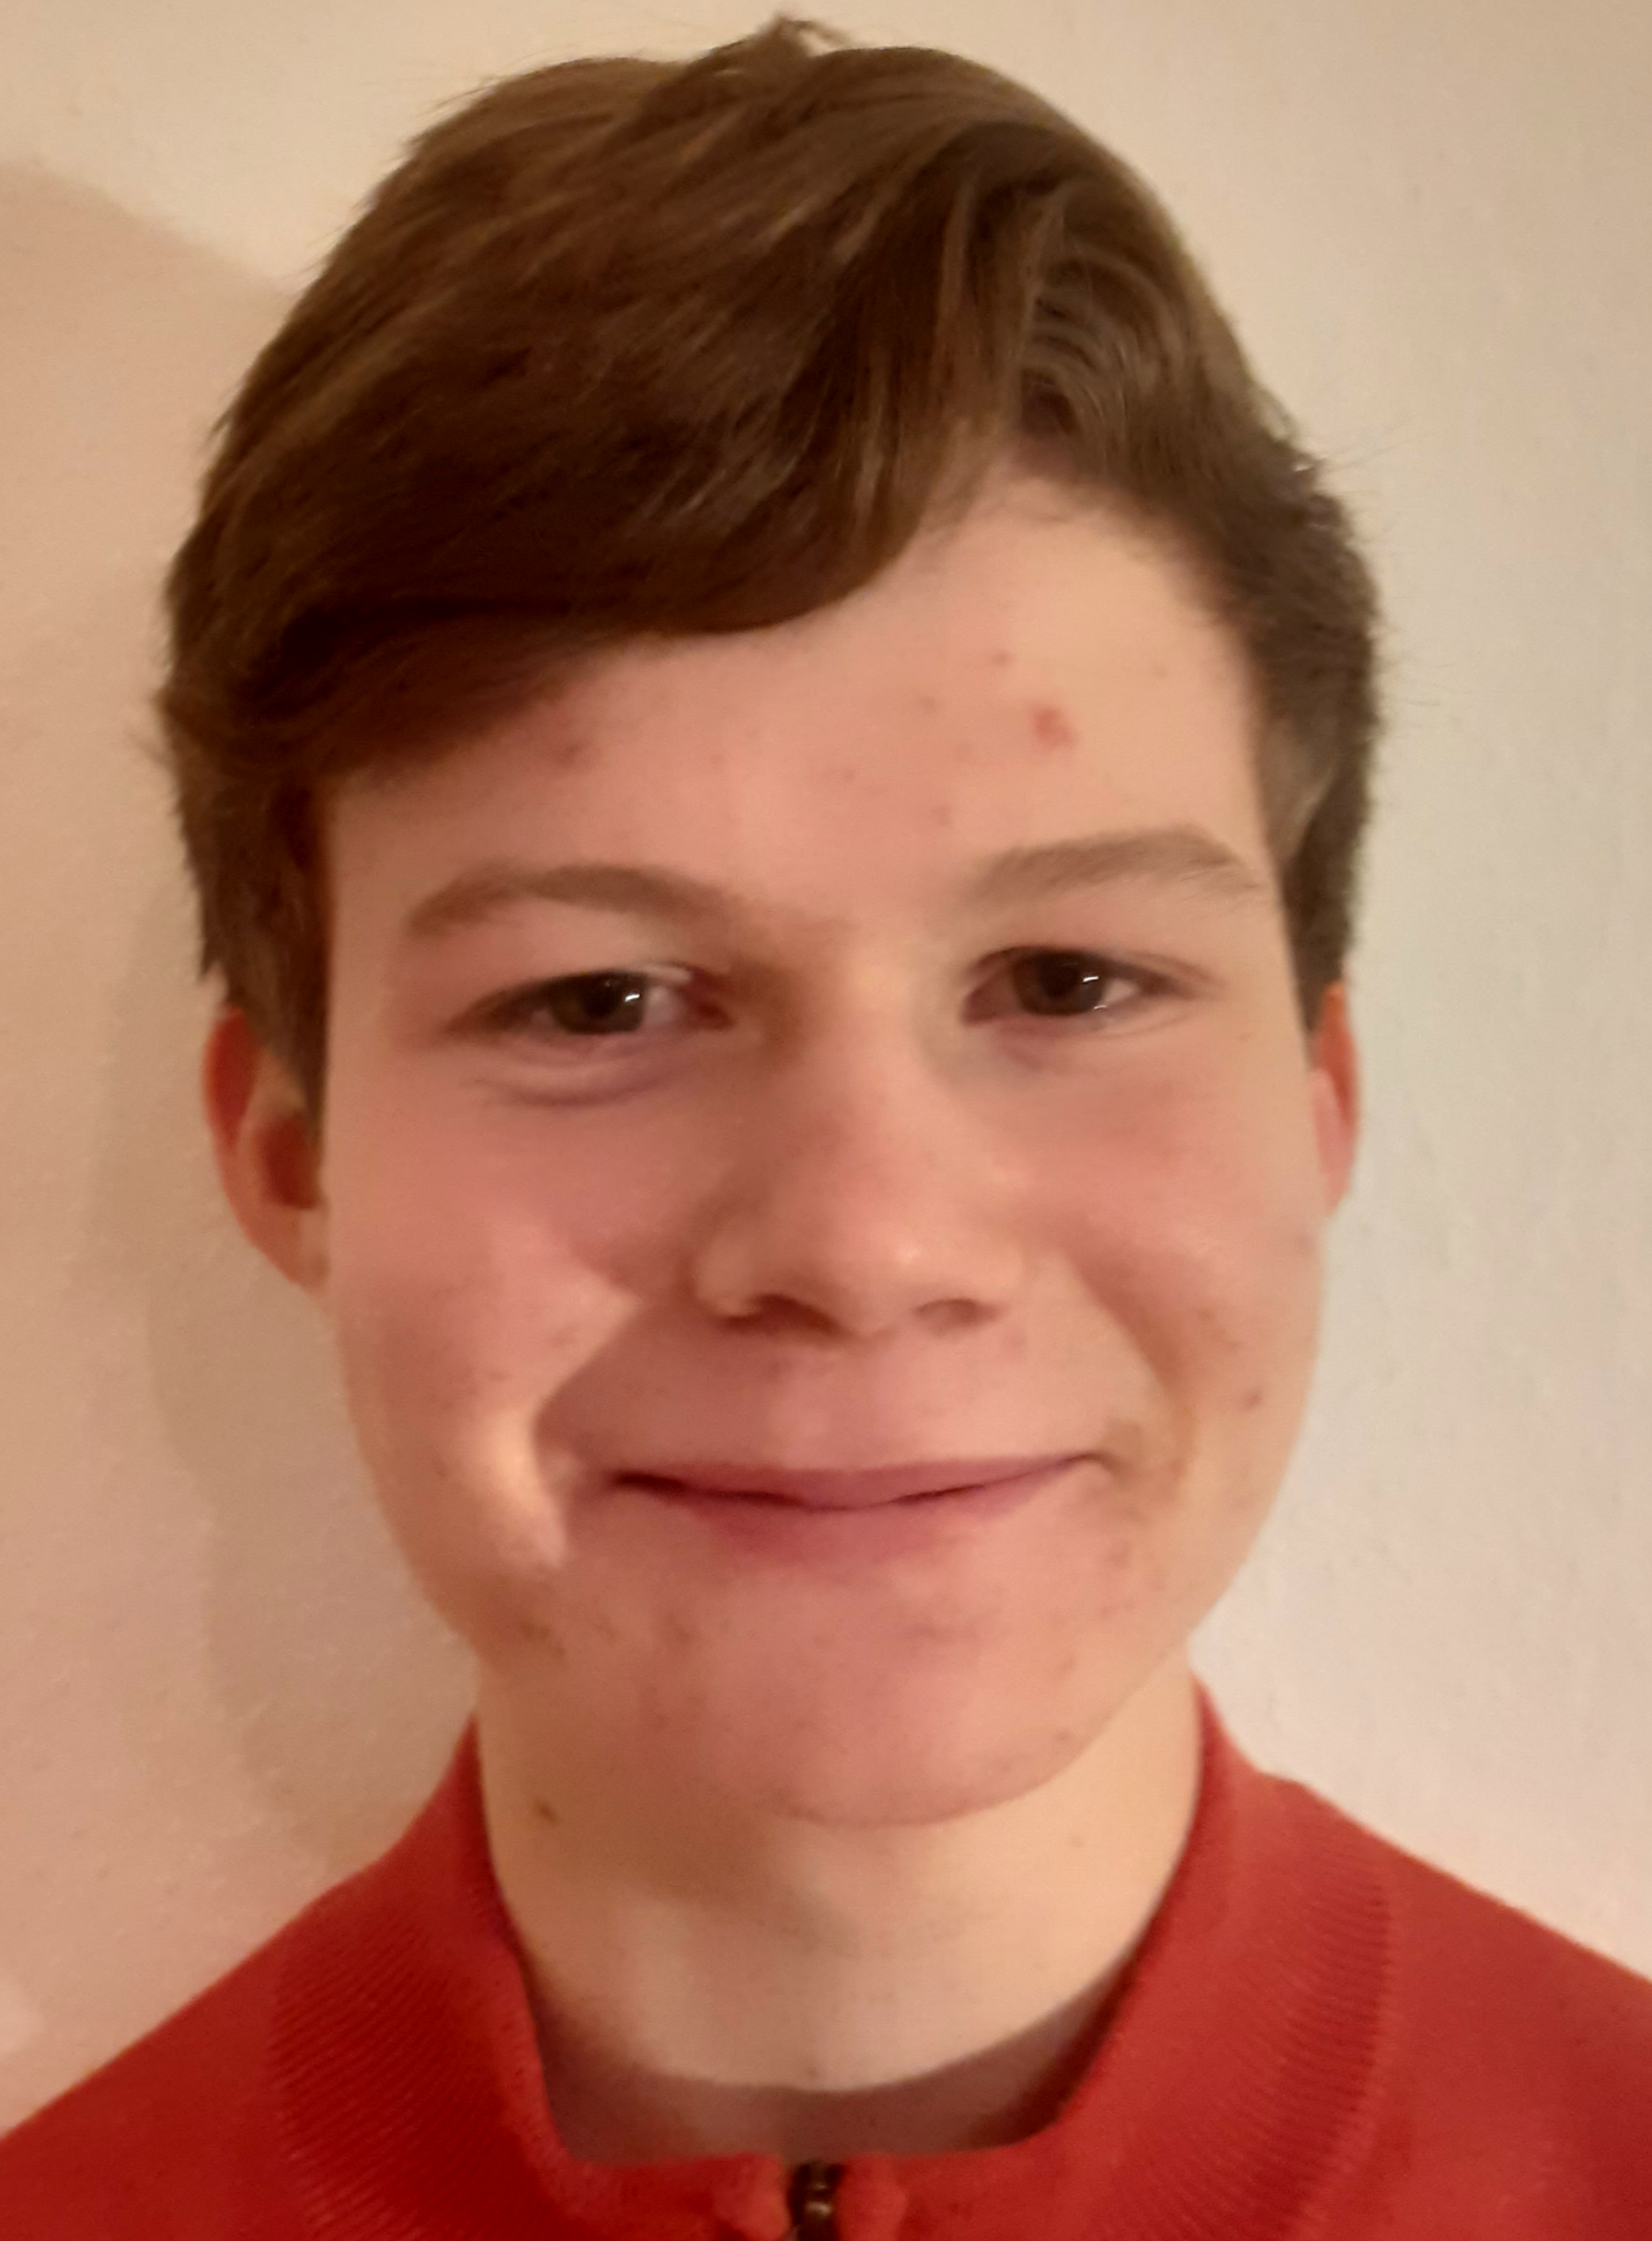
\includegraphics[trim=-50 -100 0 0mm, scale=0.05]{picture-cropped.png}
  \end{minipage}
\end{figure}
\vspace{-30pt}

\sect{Profil}

\textbf{Sch{\"u}ler der 10. Klasse an der Munich International School \\
  Angestrebter Abschluss: International Baccalaureate im Juni 2022}

\begin{itemize}[leftmargin=*]
  \itemsep0pt

\item Schulischer Schwerpunkt in Mathematik und Physik mit Kursen in \textit{\glqq
  Advanced Mathematics\grqq} und \textit{\glqq Extended Science\grqq}

\item Programmieren seit 7 Jahren als Hobby mit fortgeschrittenen Kenntnissen in
  Python und Rust

\item Musik und Sport: Gitarre seit 10 Jahren als intensives Hobby,
  Tischtennis Vereinsspieler

\item Sonstige Interessen: Freiwillige Feuerwehr und Sportklettern

\end{itemize}
\vspace{-24pt}

\sect{Schullaufbahn}
\vspace{6pt}

\iffalse
% \hspace{-\mymargin}\begin{tabularx}{\paperwidth}{p{\dimexpr0.12\linewidth}|p{\linewidth}}
\begin{tabularx}{\paperwidth}{p{0.12\linewidth}|p{0.8\linewidth}}
  % \textbf{\small \hfill Seit 2014} & \textbf{Middle und Senior School der Munich International School} \\
  \textbf{\small Seit 2014} & \textbf{Middle und Senior School der Munich International School} \\

  & \begin{itemize}[leftmargin=*]
      \itemsep3pt
      \vspace{-18pt}

    \item Fachliche Schwerpunkte: \glqq Advanced Math\grqq, \glqq Science
      Extension\grqq\, (erweiterte Physik, Chemie und Biologie, 3 Stunden zus. pro
      Woche) und Musik, 3 Stunden pro Woche
    
    \item \glqq Head of School's List\grqq\, in der 5., 6., 7., 8. und 9. Klasse
      (Auszeichnung f{\"u}r die Jahrgangsbesten mit einer Durchschnittsnote von
      mindestens 6,5 auf einer Skala von 0 bis 7)
    
    \item Schuljahrbegleitendes \textit{\glqq Personal project\grqq} (10. Klasse):
      Programmieren einen 3D-Renderer in Rust mit Fokus auf effiziente Nutzung
      des Grafikprozessors und Memory-Safety
    
    \item Programmierung einer Live-Demonstration f{\"u}r eine Veranstaltung mit
      Eltern und Sponsoren der Schule: bewegungsbesteuertes elektronisches
      Musikinstrument (Teilnehmer k{\"o}nnten durch Bewegung vor
      einem Green-Screen Ton und Lautst{\"a}rke steuern)

    \vspace{-18pt}
    \end{itemize}
  \\
  & \\[-6pt]
  \hline
  & \\[-6pt]
  
  % \textbf{\small \hfill 2011-2014} & \textbf{Dreij{\"a}hrige Segelreise von der US Ostk{\"u}ste nach Australien} \\
  \textbf{\small 2011-2014} & \textbf{Dreij{\"a}hrige Segelreise von der US Ostk{\"u}ste nach Australien} \\

  & \begin{itemize}[leftmargin=*]
      \itemsep3pt
      \vspace{-18pt}

    \item Homeschooling durch die Eltern an Bord eines Segelbootes (2. - 4. Klasse,
      ausgew{\"a}hlte Schulprojekte unter \link{namaniatsea.org/nicky-page})

    \item Unterst{\"u}tzung meiner Eltern bei Navigation und Position-plotting

      \vspace{-18pt}
    \end{itemize} \\
  & \\[-6pt]
  \hline
  & \\[-6pt]

  % \textbf{\small \hfill 2010-2011} & \textbf{1. Klasse der Munich International School}
  \textbf{\small 2010-2011} & \textbf{Grundschule der Munich International School}
\end{tabularx}
\fi

\textbf{Middle und Senior School der Munich International School} \hfill{\textit{\textbf{seit 2014}}}

\vspace{-6pt}
\begin{itemize}[leftmargin=*]
  \itemsep3pt

\item Fachliche Schwerpunkte: \glqq Advanced Math\grqq, \glqq Science
  Extension\grqq\, (erweiterte Physik, Chemie und Biologie, 3 Stunden zus. pro
  Woche) und Musik, 3 Stunden pro Woche
  
\item \glqq Head of School's List\grqq\, in der 5., 6., 7., 8. und 9. Klasse
  (Auszeichnung f{\"u}r die Jahrgangsbesten mit einer Durchschnittsnote von
  mindestens 6,5 auf einer Skala von 0 bis 7)
  
\item Schuljahrbegleitendes \textit{\glqq Personal project\grqq} (10. Klasse):
  Programmieren einen 3D-Renderer in Rust mit Fokus auf effiziente Nutzung
  des Grafikprozessors und Memory-Safety
  
\item Programmierung einer Live-Demonstration f{\"u}r eine Veranstaltung mit
  Eltern und Sponsoren der Schule: bewegungsbesteuertes elektronisches
  Musikinstrument (Teilnehmer k{\"o}nnten durch Bewegung vor
  einem Green-Screen Ton und Lautst{\"a}rke steuern)
\end{itemize}
\vspace{-6pt}

\textbf{Dreij{\"a}hrige Segelreise von der US Ostk{\"u}ste nach Australien} \hfill{\textit{\textbf{2011-2014}}}

\vspace{-18pt}
\begin{itemize}[leftmargin=*]
  \itemsep3pt

\item Homeschooling durch die Eltern an Bord eines Segelbootes (2. - 4. Klasse,
  ausgew{\"a}hlte Schulprojekte unter \link{namaniatsea.org/nicky-page})

\item Unterst{\"u}tzung meiner Eltern bei Navigation und Position-plotting

\end{itemize}
\vspace{-6pt}

\textbf{Grundschule der Munich International School} \hfill{\textit{\textbf{2010-2011}}}

\pagebreak

\sect{Kenntnisse}
\textbf{Sprachen} \hfill{Englisch (Muttersprache) und Deutsch flie{\ss}end} \\
\hspace*{\fill}Spanisch seit 4 Jahren als Fremdsprache \\
\sep
\vspace{12pt}

\textbf{Programmiersprachen} \\
\textit{Sehr gut} \hfill{Python, Rust} \\
\sep
\textit{Gut} \hfill{C/C++, Unix-Shell (bash/zsh), Lua, \LaTeX} \\
\sep
\textit{Grundkenntnisse} \hfill{Lisp, Perl, Intel-Assembly (NASM)} \\
\sep
\vspace{12pt}

{
  \small
  \textbf{Github-Repos} \hfill{3D-Renderer, Rust: \link{github.com/cynic64/render-engine}} \\
  \hspace*{\fill} Bewegungsbesteuerter Theremin, Python: \link{github.com/cynic64/theremin} \\
  \hspace*{\fill} Window-Manager Konfiguration, Lua:
  \link{github.com/cynic64/awesome-configs} \\
}
\sep
\vspace{12pt}

\textbf{Software Anwendungen} \\
\textit{Sehr gut} \hfill{MS Word, Emacs und Vi Editoren, Blender 3D Modelling Software} \\
\sep
\textit{Gut} \hfill{MS Excel, MS PowerPoint, Git} \\
\sep
\vspace{12pt}

\sect{Mitgliedschaften}

\textbf{Seit 2018} \hfill{Freiwillige Feuerwehr Gelting} \\
\sep
\textbf{Seit 2017} \hfill{Tischtennis BCF Wolfratshausen} \\
\sep
\textbf{Seit 2017} \hfill{Tischtennis SV Gelting}

\end{document}

